\chapter{تقنيات المختبر 2: التخليق والتحليل عمليًا}\label{ch:b2:lab-techniques-2}

يفشل تفاعل غرينيار صباح يوم اثنين: فالدورق كان قد شُطف لكنه لم يُجفَّف، والقطرات القليلة من
الماء الباقية فيه أتلفت الكاشف حال تكوّنه. وإذا أُعيد في أدوات زجاجية مجففة في فرن،
تحت النيتروجين، مع إضافة الهاليد قطرةً قطرة في دورق محرَّك ومبرَّد، نجح التفاعل
نفسه. فالكيمياء لم تتغير؛ بل تغيّر التركيب. ويتناول هذا الفصل الممارسة التي تحوّل
تفاعلًا على الورق إلى ناتج في قارورة: التحكم في التفاعل، وإبعاد الهواء والماء،
ومعالجته اللاحقة، وتنقيته وإثبات هوية ما صُنع.

\begin{omfigure}
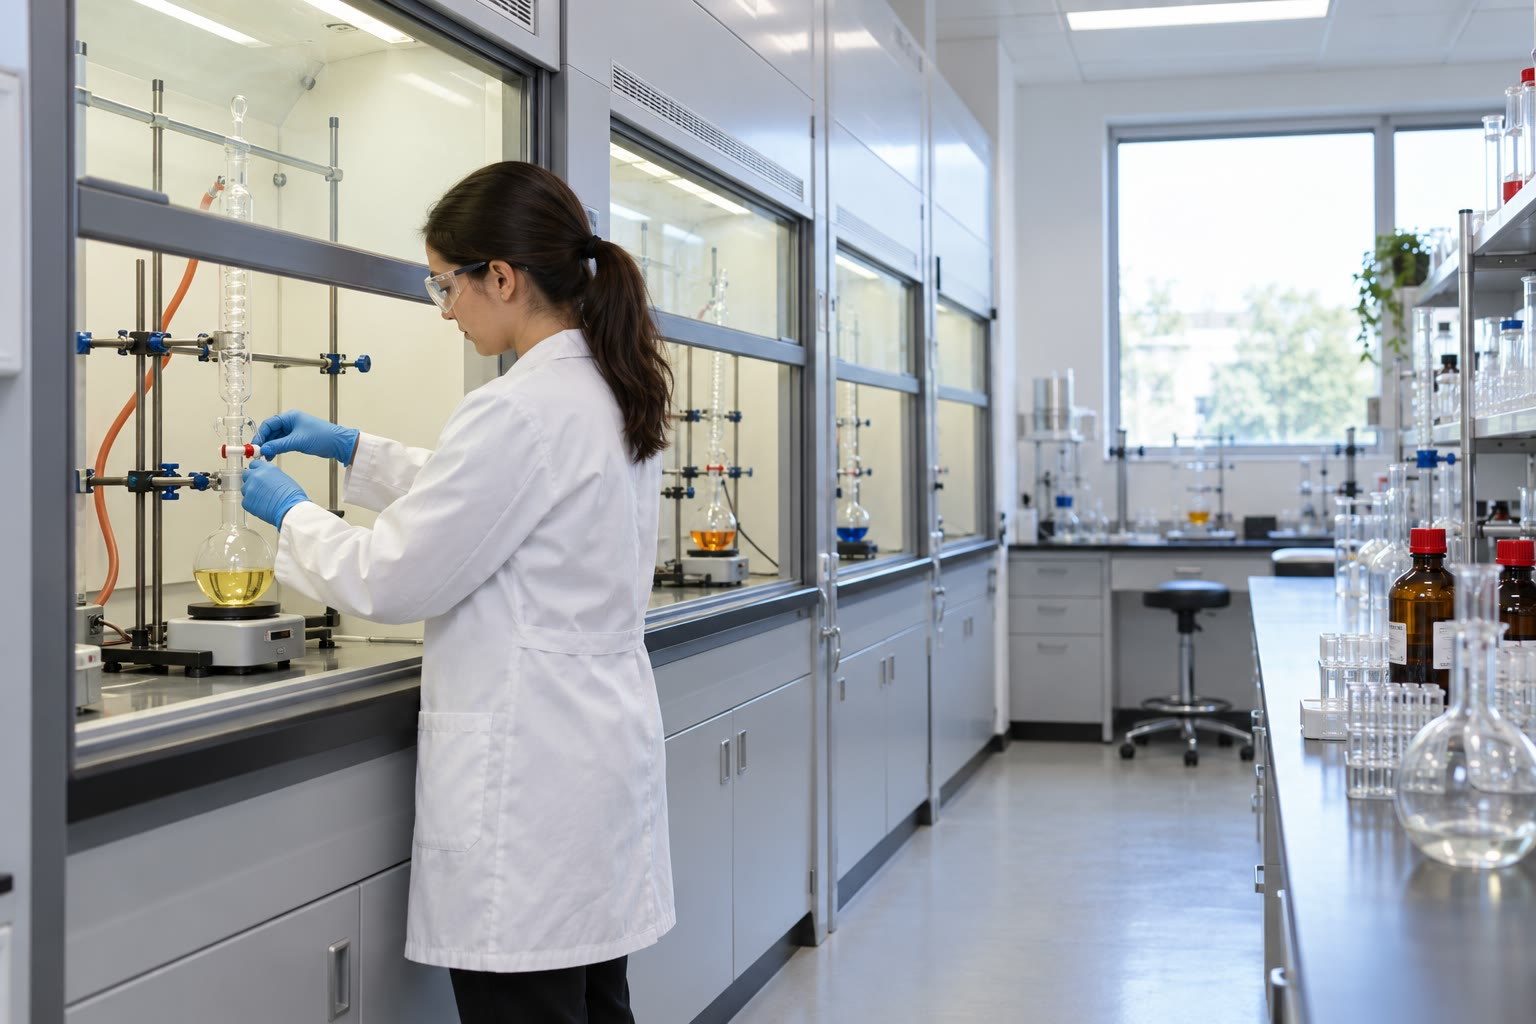
\includegraphics[width=0.56\linewidth]{images/book3/ai/b2-35-synthesis-lab.jpg}

{\small مختبر للتخليق العضوي: تفاعلات تجري تحت ساحبات الأبخرة، ودوارق مثبتة على حوامل
(رسم توضيحي).}
\end{omfigure}

\begin{recall}
مجلد السنة الأولى: المخاطر ولصائق GHS، والاستخلاص، وإعادة التبلور، والتقطير، \omterm{def:b2:chromatography:principle}{والكروماتوغرافيا}
على طبقة رقيقة و$R_f$، ونقطة الانصهار، وكواشف غرينيار. و\cref{ch:b2:reaction-enthalpy}: \omterm{def:b2:reaction-enthalpy:reaction-quantity}{أنتالبي
التفاعل} \omterm{def:b2:continuous-reactors:adiabatic-rise}{والارتفاع الكظوم لدرجة الحرارة}. و\cref{ch:b2:chromatography}،
و\cref{ch:b2:structure-determination} و\cref{ch:b2:measurement-statistics}: التحليل.
\end{recall}

\section{إجراء تفاعل تحت السيطرة}

يطلق التفاعل في الدورق حرارته حيث يحدث. ويتحكم الكيميائي في درجة الحرارة بحمام
(جليد وماء، أو جليد وملح، أو جليد جاف وأسيتون لأدنى درجات الحرارة)، وبارتداد
مذيب يغلي، الذي يحد درجة الحرارة عند درجة غليانه بينما يعيد المكثف
البخار، وبالسرعة التي يُضاف بها الكاشف. ومقياس الحرارة الداخلي، المغمور في السائل لا
في الحمام، يقيس ما يهم.

\begin{proposition}[التراكم]\label{prop:b2:lab-techniques-2:accumulation}
إذا أُضيف كاشف أسرع مما يتفاعل، تراكمت الكمية غير المتفاعلة $n_{\mathrm{acc}}$. فإن
تفاعلت بعد ذلك دفعة واحدة، بلا تبريد، ارتفعت درجة حرارة الخليط ذي السعة الحرارية $C$ بمقدار
\begin{equation*}
\Delta T_{\mathrm{ad}} = \frac{n_{\mathrm{acc}}\,|\Delta_rH|}{C}.
\end{equation*}
\end{proposition}

\begin{proof}
يطلق تفاعل $n_{\mathrm{acc}}$ الحرارة $n_{\mathrm{acc}}|\Delta_rH|$ عند ضغط ثابت
(\cref{ch:b2:reaction-enthalpy})؛ ودون تبادل حراري، تسخّن كلها الخليط، كما في
\omterm{def:b2:reaction-enthalpy:flame-temperature}{درجة حرارة اللهب الكظومة} (\cref{def:b2:reaction-enthalpy:flame-temperature}): $C\Delta T =
n_{\mathrm{acc}}|\Delta_rH|$.
\end{proof}

يكون الخطر أكبر ما يكون حين يبطؤ التفاعل في البدء، كما هو حال تكوين كواشف غرينيار غالبًا: فالهاليد المضاف
قبل البدء يتكدس، وحين يبدأ التفاعل أخيرًا يجمح. والقاعدة أن تُضاف كمية صغيرة
أولًا، ويُشاهد بدء التفاعل (تسخن، وتعكّر، وارتداد لطيف)، ثم يُضاف الباقي بالسرعة
التي يستطيع التبريد مجاراتها.

\section{الظروف الجافة والجو الخامل}

\begin{definition}[الجو الخامل]\label{def:b2:lab-techniques-2:inert}
يُجرى التفاعل تحت \emph{جو خامل}\index{جو خامل} حين يُستبدل بالهواء في الجهاز
غاز غير متفاعل، النيتروجين أو الأرغون، يُحفظ عند ضغط زائد طفيف بحيث لا
يستطيع الهواء الدخول.
\end{definition}

الكواشف العضوية الفلزية، وهيدريدات الفلزات وكثير من الحفازات تتفاعل مع الماء والأكسجين. فتُجفف الأدوات
الزجاجية في فرن وتُجمع ساخنة، أو تُلهَّب تحت تيار من الغاز؛ وتُشترى المذيبات جافة أو تُجفف
على كاشف يتفاعل مع الماء؛ وتُنقل السوائل بمحاقن عبر حواجز مطاطية.
ويغادر الغاز عبر فقاعة زيتية، تبيّن التدفق وتمنع الهواء من العودة. أما
خط شلنك وصندوق القفازات، للمركبات الأشد حساسية، فيأتيان في مجلد السنة الثالثة.

\begin{omfigure}
\begin{tikzpicture}[lab/.style={font=\scriptsize, align=center}]
\fill[omDef!10] (-1.7,-0.3) rectangle (1.7,1.0);
\draw[om glass] (-1.7,1.2) -- (-1.7,-0.3) -- (1.7,-0.3) -- (1.7,1.2);
\foreach \x/\y in {-1.5/0.0,-1.45/0.55,1.3/0.05,1.3/0.6,-1.25/0.3,1.05/-0.15}{
  \draw[omDef!50, fill=white] (\x,\y) rectangle ++(0.18,0.18);}
\pic (f) at (0,0) {threeneck={0.35}{omThm!25}};
\pic[rotate=25] (d) at (f-l) {dropfunnel={0.5}{omMeth!20}};
\pic (c) at (f-c) {condenser};
\pic[rotate=-25] (t) at (0.0,0.42) {thermometer};
\pic (b) at (3.6,3.6) {bubbler};
\draw[thick, black!60] (0,6.25) -- (0,6.75) -- (3.25,6.75) -- (b-in);
\coordinate (dtop) at ($(f-l)+(-1.52,3.26)$);
\draw[thick, black!60] (dtop) -- ++(0,0.35) -- ++(-0.9,0) node[left, lab] {N$_2$};
\node[lab, anchor=north] at (0,-0.4) {حمام جليد};
\node[lab, anchor=east] at (-1.9,2.6) {قمع\\الإضافة};
\node[lab, anchor=west] at (0.55,5.0) {مكثف};
\node[lab, anchor=west] at (1.75,2.6) {\shortstack{\foreignlanguage{arabic}{مقياس حرارة}\\\foreignlanguage{arabic}{(داخلي)}}};
\node[lab, anchor=north] at (3.6,3.45) {\shortstack{\foreignlanguage{arabic}{فقاعة (خروج الغاز)}}};
\end{tikzpicture}
\par\vspace{4pt}

{\small تفاعل تحت النيتروجين (رسم تخطيطي). دورق ثلاثي الأعناق في حمام جليد، مع مقياس حرارة
داخلي في السائل؛ ويُضاف الكاشف من قمع متساوي الضغط يدخل عبره
النيتروجين؛ ويغادر الغاز عبر المكثف وفقاعة زيتية.}
\end{omfigure}

\begin{method}[تركيب تفاعل جاف تحت النيتروجين]\label{met:b2:lab-techniques-2:anhydrous}
\begin{enumerate}
  \item جفف الأدوات الزجاجية في فرن واجمعها ساخنة، مع تشحيم الوصلات أو تغليفها؛ وركّب حاجزًا
        أو قمع الإضافة، والمكثف والفقاعة.
  \item اشطفها بالنيتروجين أثناء تبردها؛ وحافظ على تدفق بطيء (فقاعة كل ثانية أو ثانيتين) طوال العمل.
  \item أضف الأجسام الصلبة قبل الشطف، والمذيبات الجافة والكواشف السائلة بمحقنة أو بقُنية عبر
        حاجز.
  \item برّد أو سخّن كما هو مخطط؛ وابدأ الإضافة بكمية صغيرة وتحقق من أن التفاعل
        بدأ قبل المتابعة.
\end{enumerate}
\end{method}

\section{المعالجة اللاحقة}

\begin{definition}[المعالجة اللاحقة]\label{def:b2:lab-techniques-2:work-up}
\emph{المعالجة اللاحقة}\index{معالجة لاحقة} لتفاعل هي سلسلة العمليات، بعد التفاعل، التي
تحوّل خليط التفاعل إلى الناتج الخام: الإخماد، والاستخلاص والغسل، والتجفيف،
والترشيح وتبخير المذيب.
\end{definition}

\begin{definition}[الاستخلاص حمض--قاعدة]\label{def:b2:lab-techniques-2:acid-base-extraction}
\emph{الاستخلاص حمض--قاعدة}\index{استخلاص حمض--قاعدة} يفصل المركبات العضوية الحمضية والقاعدية والمتعادلة
المذابة في مذيب عضوي بغسل المحلول بأحماض أو قواعد مائية،
تحوّل صنفًا واحدًا من المركبات إلى أيونات تنتقل إلى الماء.
\end{definition}

\begin{proposition}[من يذهب إلى أين]\label{prop:b2:lab-techniques-2:acid-base-extraction}
يستخلص هيدروجين كربونات الصوديوم المائي (pH 8.3) حمضًا كربوكسيليًا ($\mathrm pK_a$ نحو 4) لكنه لا يستخلص
فينولًا ($\mathrm pK_a$ نحو 10)، الذي يحتاج إلى هيدروكسيد الصوديوم؛ ويستخلص حمض الهيدروكلوريك المخفف
أمينًا لحمضه المرافق $\mathrm pK_a$ قدره 4.6 أو أكثر؛ وتبقى المركبات المتعادلة في الطبقة
العضوية.
% ledger: ph:NaHCO3, pka:benzoic, pka:phenol, pka:anilinium
\end{proposition}

\begin{proof}
يكون النوع في صورته القاعدية أساسًا حين $\mathrm{pH} > \mathrm pK_a$، وبنسبة تتجاوز 99~\% حين
$\mathrm{pH} > \mathrm pK_a + 2$. فعند pH 8.3، يكون حمض البنزويك (4.2) بنزوات بنسبة تتجاوز 99~\%، وهو أيون
يبقى في الماء؛ أما الفينول (9.99) فنحو 2~\% منه فينوكسيد ($10^{8.3 - 10.0}$) ويبقى أساسًا
في الطبقة العضوية، حيث تتوزع الصورة المتعادلة. وفي هيدروكسيد الصوديوم (pH فوق 12) يتحول الفينول
إلى فينوكسيد. وفي حمض الهيدروكلوريك المخفف (pH نحو 1)، يكون الأنيلين (أنيلينيوم 4.6) أنيلينيومًا بنسبة تتجاوز
99~\%. وكل أيون، حين يصير في الماء، يُستعاد بإرجاع pH في الاتجاه الآخر، مما
يجدد المركب المتعادل، ثم باستخلاصه من جديد.
\end{proof}

\begin{omfigure}
\begin{tikzpicture}[x=1cm, y=1cm, st/.style={draw=black!70, rounded corners=2pt, fill=white,
  font=\scriptsize, align=center, inner sep=3pt, text width=3.0cm}, ar/.style={->, thick, black!70}]
\node[st, fill=omDef!10] (m) at (0,0) {\foreignlanguage{arabic}{حمض البنزويك، الفينول،}\\\foreignlanguage{arabic}{الأنيلين، النفثالين}\\\foreignlanguage{arabic}{في الإيثوكسي إيثان}};
\node[st, fill=omThm!10] (a1) at (5.0,0) {\foreignlanguage{arabic}{مائي: بنزوات}\\\babelsublr{$\to$ HCl $\to$ \foreignlanguage{arabic}{حمض البنزويك}}};
\node[st] (o1) at (0,-1.6) {\foreignlanguage{arabic}{الفينول، الأنيلين،}\\\foreignlanguage{arabic}{النفثالين}};
\node[st, fill=omThm!10] (a2) at (5.0,-1.6) {\foreignlanguage{arabic}{مائي: فينوكسيد}\\\babelsublr{$\to$ HCl $\to$ \foreignlanguage{arabic}{فينول}}};
\node[st] (o2) at (0,-3.2) {\foreignlanguage{arabic}{الأنيلين، النفثالين}};
\node[st, fill=omThm!10] (a3) at (5.0,-3.2) {\foreignlanguage{arabic}{مائي: أنيلينيوم}\\\babelsublr{$\to$ NaOH $\to$ \foreignlanguage{arabic}{أنيلين}}};
\node[st, fill=omMeth!10] (o3) at (0,-4.8) {\shortstack{\foreignlanguage{arabic}{النفثالين}\\\foreignlanguage{arabic}{(جفف، وبخّر)}}};
\draw[ar] (m) -- node[above, font=\tiny] {\foreignlanguage{arabic}{غسل \babelsublr{NaHCO$_3$}}} (a1);
\draw[ar] (m) -- (o1); \draw[ar] (o1) -- node[above, font=\tiny] {\foreignlanguage{arabic}{غسل \babelsublr{NaOH}}} (a2);
\draw[ar] (o1) -- (o2); \draw[ar] (o2) -- node[above, font=\tiny] {\foreignlanguage{arabic}{غسل \babelsublr{HCl}}} (a3);
\draw[ar] (o2) -- (o3);
\pic at (8.6,-3.6) {sepfunnel={omDef!25}{omThm!20}};
\node[font=\scriptsize, align=center] at (8.6,-4.0) {قمع الفصل};
\end{tikzpicture}
\par\vspace{4pt}

{\small الفصل حمض--قاعدة لأربعة مركبات (\cref{prop:b2:lab-techniques-2:acid-base-extraction}).
تفقد الطبقة العضوية (العمود الأيسر) صنفًا واحدًا عند كل غسل؛ ويعيد كل مستخلص مائي (يمينًا)
مركبه حين يُعكس pH.}
\end{omfigure}

\begin{definition}[عامل التجفيف]\label{def:b2:lab-techniques-2:drying-agent}
\emph{عامل التجفيف}\index{عامل تجفيف} ملح لامائي، مثل كبريتات المغنيزيوم أو كبريتات الصوديوم،
يربط الماء المذاب في محلول عضوي على هيئة ماء تبلور ثم يُزال
بالترشيح.
\end{definition}

\begin{method}[من دورق التفاعل إلى الناتج الخام]\label{met:b2:lab-techniques-2:work-up}
\begin{enumerate}
  \item الإخماد: أتلف الكواشف التفاعلية المتبقية بمحلول مائي مناسب، ببطء ومع
        التبريد.
  \item استخلص في مذيب عضوي؛ وافصل الطبقتين (وتحقق من هوية كل منهما بإضافة قطرة
        ماء)؛ واستخلص الطبقة المائية من جديد.
  \item اغسل الطبقات العضوية المجمّعة (حمض، ثم قاعدة، ثم المحلول الملحي، وهو محلول مشبع من كلوريد الصوديوم
        يزيل معظم الماء المذاب).
  \item جفف \omterm{def:b2:lab-techniques-2:drying-agent}{بعامل تجفيف} حتى يبقى بعضه حرّ الانسياب؛ ثم رشّح.
  \item أزل المذيب في مبخر دوّار تحت ضغط مخفَّض؛ وزن الناتج الخام.
\end{enumerate}
\end{method}

\section{التنقية}

\begin{definition}[الكروماتوغرافيا الومضية]\label{def:b2:lab-techniques-2:flash}
\emph{الكروماتوغرافيا الومضية}\index{كروماتوغرافيا ومضية} \omterm{def:b2:chromatography:principle}{كروماتوغرافيا} عمودية تحضيرية على السيليكا
يُدفع فيها المُزيح عبر العمود بضغط غاز طفيف، بحيث لا يستغرق فصل غرامات
من المادة إلا دقائق؛ ويُختار المُزيح \omterm{def:b2:chromatography:principle}{بالكروماتوغرافيا} على طبقة رقيقة على السيليكا نفسها.
\end{definition}

\begin{proposition}[حجوم العمود]\label{prop:b2:lab-techniques-2:column-volumes}
المركب الذي يسير بقيمة $R_f$ على صفيحة TLC يغادر عمودًا من السيليكا والمُزيح نفسيهما بعد
نحو $1/R_f$ حجمًا عموديًا من المُزيح.
\end{proposition}

\begin{proof}[تعليل]
على الصفيحة يقطع المركب $R_f$ ضعفًا من المسافة التي تقطعها جبهة المذيب: فسرعته المتوسطة $R_f$
ضعفًا من سرعة المُزيح. وعلى العمود يعطي التوزع نفسه النسبة نفسها بين السرعتين، فيحتاج
المركب إلى $1/R_f$ ضعفًا من حجم المُزيح الذي يملأ العمود (الحجم الميت) ليخرج؛
وبلغة \cref{ch:b2:chromatography}، $R_f \approx 1/(1 + k)$. فالمركب ذو $R_f = 0.25$
يخرج بعد نحو أربعة حجوم عمودية، منفصلًا جيدًا عن مركب عند 0.5 (حجمان).
\end{proof}

\begin{omfigure}
\begin{tikzpicture}[lab/.style={font=\scriptsize, align=left, anchor=west}]
\pic (k) at (0,0) {chromcolumn={3.4}};
\node[lab] at (0.6,4.6) {مُزيح};
\node[lab] at (0.6,3.55) {رمل};
\node[lab] at (0.6,2.2) {طبقة السيليكا};
\foreach \i/\c in {0/white, 1/omThm!25, 2/omThm!25, 3/white, 4/omDef!25, 5/omDef!25, 6/white}{
  \pic at ({2.4+0.55*\i},-1.2) {testtube={0.45}{\c}};}
\node[font=\scriptsize] at (4.05,-1.6) {\foreignlanguage{arabic}{الأجزاء من 1 إلى 7}};
\pic at (7.6,-1.2) {tlcplate};
\foreach \j/\x in {2/7.15,3/7.45,5/7.75,6/8.05}{\node[font=\tiny] at (\x,-1.38) {\j};}
\fill[omThm] (7.45,0.95) circle (0.06); \fill[omThm] (7.15,0.95) circle (0.06);
\fill[omDef] (8.05,-0.05) circle (0.06); \fill[omDef] (7.75,-0.05) circle (0.06);
\node[font=\scriptsize, align=center] at (7.6,2.15) {\babelsublr{TLC}\\للأجزاء};
\end{tikzpicture}
\par\vspace{4pt}

{\small \omterm{def:b2:lab-techniques-2:flash}{الكروماتوغرافيا الومضية} (رسم تخطيطي). يُحمَّل الناتج الخام فوق السيليكا ويُزاح؛
ويُجمع السائل الخارج في أجزاء؛ وتبيّن صفيحة TLC للأجزاء أين خرج كل مركب
(هنا المركب السريع غير القطبي في الجزأين 2--3، والأبطأ في 5--6)، وتُجمع الأجزاء النقية.}
\end{omfigure}

\begin{method}[تشغيل عمود ومضي]\label{met:b2:lab-techniques-2:flash}
\begin{enumerate}
  \item اختر المُزيح \omterm{def:b2:chromatography:principle}{بكروماتوغرافيا} TLC: المركب المطلوب عند $R_f$ نحو 0.25--0.35، وأبعد ما يمكن عن
        الشوائب.
  \item احشُ السيليكا (نحو 30 إلى 100 ضعف كتلة الناتج الخام) على هيئة عجينة أو جافة؛ وأضف طبقة
        من الرمل.
  \item حمّل الناتج الخام في أقل حجم من المذيب (أو ممتزًا على قليل من السيليكا).
  \item أزح تحت ضغط طفيف؛ واجمع الأجزاء؛ وافحصها \omterm{def:b2:chromatography:principle}{بكروماتوغرافيا} TLC؛ واجمع النقية منها ثم
        بخّرها.
\end{enumerate}
\end{method}

تُقطَّر السوائل التي تتفكك قرب درجة غليانها تحت ضغط مخفَّض، حيث تغلي
عند درجة أدنى.

\begin{definition}[التقطير تحت ضغط مخفَّض]\label{def:b2:lab-techniques-2:reduced-pressure}
\emph{التقطير تحت ضغط مخفَّض}\index{تقطير تحت ضغط مخفض} يُجرى
في جهاز موصول بمضخة تفريغ عبر مقياس ضغط، عند ضغط يغلي فيه السائل عند
درجة حرارة يتحملها.
\end{definition}

\begin{proposition}[الغليان تحت ضغط مخفَّض]\label{prop:b2:lab-techniques-2:reduced-pressure}
مع $T_b$ درجة حرارة الغليان عند الضغط المرجعي $p^\circ$ و$\Delta_{\mathrm{vap}}H$
معاملًا على أنه ثابت، تُعطى درجة حرارة الغليان عند الضغط $p$ بالعلاقة
\begin{equation*}
\frac{1}{T} = \frac{1}{T_b} - \frac{R}{\Delta_{\mathrm{vap}}H}\ln\frac{p}{p^\circ}.
\end{equation*}
\end{proposition}

\begin{proof}
يغلي السائل حين يساوي ضغط بخاره الضغط فوقه. وعلاقة كلاوزيوس--كلابيرون
المعروفة في الفيزياء، $\mathrm d\ln p/\mathrm dT = \Delta_{\mathrm{vap}}H/(RT^2)$ من أجل بخار مثالي 
وحجم سائل مهمل، إذا كوملت بين $(T_b, p^\circ)$ و$(T, p)$ أعطت $\ln(p/p^\circ) =
-(\Delta_{\mathrm{vap}}H/R)(1/T - 1/T_b)$؛ وإعادة الترتيب تعطي النتيجة.
\end{proof}

\begin{omfigure}
\begin{tikzpicture}
\begin{axis}[width=0.72\linewidth, height=5.2cm, xmode=log, xmin=5, xmax=1100, ymin=0, ymax=190,
  xlabel={\foreignlanguage{arabic}{الضغط \babelsublr{(\unit{mbar})}}}, ylabel={\foreignlanguage{arabic}{درجة حرارة الغليان \babelsublr{(\unit{\degreeCelsius})}}},
  label style={font=\small}, tick label style={font=\scriptsize}, grid=major, grid style={black!10},
  legend style={font=\scriptsize, at={(0.02,0.98)}, anchor=north west}, legend cell align=left]
\addplot[omDef, thick] table[x=p, y=bromobenzene] {figdata/out/bachelor-2-vacuum-boiling.dat};
\addplot[omThm, thick] table[x=p, y=benzaldehyde] {figdata/out/bachelor-2-vacuum-boiling.dat};
\addplot[only marks, mark=o, mark size=2pt, omDef] coordinates {(7,27.75)};
\addplot[only marks, mark=o, mark size=2pt, omThm] coordinates {(13,61.85)};
\legend{بروموبنزين, بنزالدهيد, مقيسة}
\end{axis}
\end{tikzpicture}

{\small درجة حرارة الغليان بدلالة الضغط (\cref{prop:b2:lab-techniques-2:reduced-pressure}) مع
أنتالبيات التبخر ودرجات الغليان من قاعدة NIST الشبكية. والدوائر درجات غليان مقيسة
عند 7 و\qty{13}{mbar}، غير مستعملة في المنحنيين: فالمعادلة البسيطة صحيحة في حدود بضع كلفنات.
وخفض الضغط من \qty{1}{bar} إلى \qty{20}{mbar} يخفض درجات الغليان بأكثر من
\qty{100}{K}.}
% figdata: bachelor-2/vacuum-boiling.py
% ledger: tb:bromobenzene, dvap:bromobenzene, tbp:bromobenzene.7mbar, tb:benzaldehyde, dvap:benzaldehyde, tbp:benzaldehyde.13mbar
\end{omfigure}

\section{النقاوة والهوية}

يُتعرف الناتج بمقارنة أطيافه وثوابته الفيزيائية بأطياف المركب المتوقع وثوابته
(\cref{ch:b2:structure-determination})؛ وتُقاس نقاوته على حدة، لأن الناتج
قد يكون المركب الصحيح ومع ذلك يحوي بضعة بالمئة من شيء آخر.

\begin{method}[إعلان النقاوة والمردود]\label{met:b2:lab-techniques-2:purity}
\begin{enumerate}
  \item تحقق من مجال انصهار الصلب (حاد وقريب من القيمة المنشورة للمركب
        النقي) ومن كروماتوغرافياه على طبقة رقيقة (بقعة واحدة في مُزيحين).
  \item قِس النقاوة: النسبة المئوية للمساحة في GC أو HPLC (وهي تقدير فقط ما لم تكن معاملات الاستجابة معلومة،
        \cref{ch:b2:chromatography})، أو الرنين المغناطيسي النووي الكمي للبروتون، بمقارنة تكامل للناتج
        بتكامل لكل شائبة، أو \omterm{def:b2:chromatography:quantitative}{بمعيار داخلي} موزون.
  \item حوّل إلى كسر كتلي $w$ للناتج في المادة المعزولة.
  \item أعلن المردود المصحح بالنقاوة: $\rho = w\,m/(n_{\mathrm{lim}}M)$، حيث $m$
        الكتلة المعزولة، و$n_{\mathrm{lim}}$ كمية الكاشف المحدد و$M$ الكتلة المولية.
\end{enumerate}
\end{method}

ومن أجل ناتج نشط ضوئيًا، يضيف الدوران النوعي فحصًا لنقاوته الفراغية؛ أما
الفائض المرآوي وقياسه فيُعالجان في مجلد السنة الثالثة.

\begin{safety}{\ghs[5mm]{GHS02}\,\ghs[5mm]{GHS06}\,\ghs[5mm]{GHS07}\,\ghs[5mm]{GHS08}\,\ghs[5mm]{GHS09}}
الإيثوكسي إيثان والأوكسولان شديدا الاشتعال ويكوّنان فوق أكاسيد متفجرة عند التخزين؛ فلا لهب في
المختبر، وتُفحص القوارير القديمة قبل التقطير. والبروموبنزين قابل للاشتعال وسام للأحياء
المائية؛ وبُرادة المغنيزيوم قابلة للاشتعال. وتُفحص الأدوات الزجاجية للتفريغ بحثًا عن الشقوق النجمية وتُحمى بحاجز.
% ledger: ghs:ether, ghs:THF, ghs:bromobenzene, ghs:Mg, ghs:MgSO4
\end{safety}

\section{تمارين}

\begin{exercise}[$\star$]\label{exo:b2:lab-techniques-2:1}
أي حمام تستعمل لتفاعل يُجرى عند نحو \qty{0}{\degreeCelsius}، وعند نحو
\qty{-15}{\degreeCelsius}، وعند \qty{-78}{\degreeCelsius}؟
\end{exercise}

\begin{exercise}[$\star$]\label{exo:b2:lab-techniques-2:2}
يستعمل استخلاص ثنائي كلوروميثان، الأكثف من الماء. أي الطبقتين عضوية؟ وكيف تتحقق من ذلك؟
\end{exercise}

\begin{exercise}[$\star$]\label{exo:b2:lab-techniques-2:3}
كيف تعرف أن ما أُضيف من كبريتات المغنيزيوم إلى محلول إيثري كافٍ؟
\end{exercise}

\begin{exercise}[$\star$]\label{exo:b2:lab-techniques-2:4}
في الخليط 4\,:\,1 هكسان--إيثانوات الإيثيل يكون للناتج $R_f = 0.65$ وللشائبة 0.75. ماذا تغيّر
من أجل عمود، وفي أي اتجاه؟
\end{exercise}

\begin{exercise}[$\star\star$]\label{exo:b2:lab-techniques-2:5}
أعطِ ترتيب الغسلات التي تفصل حمض البنزويك والفينول والأنيلين والنفثالين من محلول
إيثري، مع تعليل كل منها بقيمة $\mathrm pK_a$، وكيف يُستعاد كل مركب.
\end{exercise}

\begin{exercise}[$\star\star$]\label{exo:b2:lab-techniques-2:6}
قدّر درجتي غليان البروموبنزين والبنزالدهيد عند \qty{20}{mbar}.
\end{exercise}

\begin{exercise}[$\star\star$]\label{exo:b2:lab-techniques-2:7}
أثناء إضافة، تراكم \qty{0.050}{mol} من كاشف دون أن يتفاعل. مع $\Delta_rH =
\qty{-200}{kJ/mol}$ وسعة حرارية للخليط قدرها \qty{400}{J/K} (معطيات تمرين)، ما
ارتفاع درجة الحرارة الذي قد يتبع ذلك؟
\end{exercise}

\begin{exercise}[$\star\star$]\label{exo:b2:lab-techniques-2:8}
يُظهر مسار HPLC الناتج عند 96.0~\% من المساحة الكلية. لماذا ليست هذه بعد نقاوة كتلية؟ 
ويُظهر طيف بروتون للعينة نفسها إشارة أحادية للناتج (1H) تكاملها 1.00 وإشارة أحادية لشائبة
(3H) تكاملها 0.12؛ والناتج \qty{200}{g/mol}، والشائبة \qty{100}{g/mol} (معطيات تمرين). احسب
الكسر الكتلي للناتج.
\end{exercise}

\begin{exercise}[$\star\star$]\label{exo:b2:lab-techniques-2:9}
يُحصل على \qty{4.10}{g} من ناتج (\qty{164}{g/mol}) نقاوته 95.0~\% (كتلةً) انطلاقًا من \qty{0.0300}{mol}
من الكاشف المحدد. احسب المردود، غير مصحح ومصححًا.
\end{exercise}

\begin{exercise}[$\star\star\star$]\label{exo:b2:lab-techniques-2:10}
أعطى تفاعل غرينيار البنزين وكاد لا يعطي أي كحول بعد إضافة الألدهيد. عدّد
الأسباب الممكنة وكيف يُتجنب كل منها.
\end{exercise}

\begin{exercise}[$\star\star\star$]\label{exo:b2:lab-techniques-2:11}
عند تكبير المقياس، يتفاعل \qty{1.00}{mol} من هاليد مع $\Delta_rH = \qty{-270}{kJ/mol}$ في مفاعل
لا يزيل تبريده أكثر من \qty{150}{W} (معطيات تمرين). ما أقصر زمن إضافة آمن؟ وماذا
يحدث إذا كانت الإضافة أسرع؟
\end{exercise}

\begin{exercise}[$\star\star\star$]\label{exo:b2:lab-techniques-2:12}
يمكن تنقية صلب خام كتلته \qty{13.0}{g} بإعادة التبلور (خطوة واحدة، استرداد 80~\%، نقاوة
99~\%) أو \omterm{def:b2:lab-techniques-2:flash}{بالكروماتوغرافيا الومضية} (استرداد 95~\%، نقاوة 99.5~\%، و\qty{1.5}{L} من المذيب) (معطيات
تمرين). قارن الطريقين.
\end{exercise}

\section{مسألة: تفاعل غرينيار كما ينبغي}

\begin{problem}[{مسألة نهاية الأسبوع --- المخاطر والتركيب الجاف، والإضافة المضبوطة 
وخطر التراكم، والمعالجة اللاحقة، والتنقية بالكروماتوغرافيا الومضية ومردود مصحح بالنقاوة}]
\label{pb:b2:lab-techniques-2:1}
معطيات تمرين. يُحضَّر بروميد فينيل المغنيزيوم من \qty{15.7}{g} من البروموبنزين و\qty{2.67}{g} من
بُرادة المغنيزيوم في الإيثوكسي إيثان الجاف، ثم يُضاف \qty{9.55}{g} من البنزالدهيد؛ وتعطي \omterm{def:b2:lab-techniques-2:work-up}{المعالجة اللاحقة}
بكلوريد الأمونيوم المائي ثنائي فينيل الميثانول. تكوين الكاشف: $\Delta_rH =
\qty{-270}{kJ/mol}$؛ والسعة الحرارية للخليط \qty{170}{J/K}؛ والبدء عند \qty{20}{\degreeCelsius}. وTLC
(9\,:\,1 هكسان--إيثانوات الإيثيل): ثنائي الفينيل $R_f = 0.85$، وثنائي فينيل الميثانول 0.25. والمعزول بعد العمود:
\qty{12.50}{g}. وفي طيف البروتون لهذه المادة: إشارة \ce{CH(OH)} الأحادية (1H) تكاملها 1.00، والمنطقة
\omterm{def:b2:huckel:aromatic}{العطرية} 10.90. والكتل المولية (\unit{g/mol}): البروموبنزين 157.01، والبنزالدهيد 106.12، وثنائي فينيل الميثانول
184.24، وثنائي الفينيل 154.21؛ وMg 24.305.
% ledger: ghs:ether, ghs:bromobenzene, ghs:Mg, ghs:benzaldehyde, ghs:NH4Cl, ghs:biphenyl, ghs:benzhydrol, tb:ether, aw:Mg, aw:C, aw:H, aw:Br, aw:O, nmr:biphenyl

\medskip
\noindent\textbf{الجزء الأول --- المخاطر والتركيب.}
\begin{enumerate}
  \item أعطِ المخاطر الرئيسية للإيثوكسي إيثان والبروموبنزين والمغنيزيوم.
  \item اكتب تفاعل بروميد فينيل المغنيزيوم مع الماء، وفسّر استعمال الأدوات الزجاجية المجففة في الفرن.
  \item لماذا العمل تحت النيتروجين؟
  \item ماذا تبيّن الفقاعة، وماذا تمنع؟
  \item لماذا يكون الإيثوكسي إيثان مذيبًا جيدًا هنا؟
  \item احسب كميتي البروموبنزين والمغنيزيوم. أيهما بفائض؟
\end{enumerate}

\medskip
\noindent\textbf{الجزء الثاني --- الإضافة المضبوطة.}
\begin{enumerate}[resume]
  \item ما الحرارة التي يطلقها التكوين التام للكاشف؟
  \item لماذا يُضاف البروموبنزين قطرةً قطرة؟
  \item يبطؤ التفاعل في البدء، ويُضاف 20~\% من البروموبنزين قبل أن يبدأ. ما الحرارة التي
        يمكن أن تنطلق حينئذ دفعة واحدة؟
  \item احسب \omterm{def:b2:continuous-reactors:adiabatic-rise}{الارتفاع الكظوم لدرجة الحرارة}.
  \item قارن درجة الحرارة النهائية بدرجة غليان الإيثوكسي إيثان. ماذا يحدث؟
  \item كيف ينبغي أن تُجرى الإضافة؟
\end{enumerate}

\medskip
\noindent\textbf{الجزء الثالث --- الإضافة \omterm{def:b2:lab-techniques-2:work-up}{والمعالجة اللاحقة}.}
\begin{enumerate}[resume]
  \item اكتب التفاعل مع البنزالدهيد وحدّد الكاشف المحدد.
  \item لماذا يُخمَد بكلوريد الأمونيوم لا بحمض قوي؟
  \item أي الطبقتين عضوية في قمع الفصل؟
  \item ما فائدة الغسل بالمحلول الملحي؟
  \item كيف يُجفف المحلول، وكيف يُزال المذيب؟
  \item ثنائي الفينيل هو الناتج الثانوي الرئيسي. كيف يتكوّن، وما الذي يحابيه؟
\end{enumerate}

\medskip
\noindent\textbf{الجزء الرابع --- التنقية والنقاوة.}
\begin{enumerate}[resume]
  \item أي المركبين يغادر العمود أولًا؟
  \item بعد كم حجمًا عموديًا يخرج كل منهما؟
  \item من تكاملات الرنين المغناطيسي النووي، احسب النسبة المولية لثنائي الفينيل إلى الكحول في المادة
        المعزولة.
  \item احسب الكسر الكتلي لثنائي فينيل الميثانول.
  \item احسب كتلة ثنائي فينيل الميثانول النقي.
  \item احسب الكتلة النظرية.
  \item احسب المردود دون تصحيح بالنقاوة.
  \item اذكر المردود المصحح بالنقاوة.
\end{enumerate}
\end{problem}
